\subsection{外代数的函子性质}

命题 2. 设 A 是一个交换环，M 和 N 是两个 A-模，u: M → N 是一个 A-线性映射。则存在唯一的 A-代数同态

\[
u ^ {\prime \prime}: \bigwedge (\mathbf {M}) \rightarrow \bigwedge (\mathbf {N})
\]

使得图表

\pandocbounded{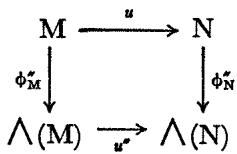
\includegraphics[keepaspectratio]{images/part003_b216bf24.jpg}}

是交换的。此外， \(u''\) 是一个分次代数同态。

\(u''\) 的存在性与唯一性由第 1 号，命题 1 应用于代数 \(\bigwedge(\mathbf{N})\) 和 \(f = \phi_{\mathbf{N}}'' \circ u: \mathbf{M} \to \bigwedge(\mathbf{N})\) 得出；因为 \(f(\mathbf{M}) \subset \mathbf{N}\) ，因此 \(f\) 由 \(\mathfrak{J}_{\mathbf{N}}''\) 的定义满足条件 (1)：由于 \(f(\mathbf{M}) \subset \bigwedge^{1}(\mathbf{N}) = \mathbf{N}\) ，\(u''\) 是分次代数同态这一事实由第 1 号的注记 1 得出。

命题 2 中的同态 \(u''\) 此后将记为 \(\bigwedge(u)\) 。若 P 是一个 A-模且 \(v: \mathbf{N} \to \mathbf{P}\) 是一个 A-线性映射，则

\[
\bigwedge (v \circ u) = \bigwedge (v) \circ \bigwedge (u)\tag{3}
\]

因为 \(\bigwedge(v) \circ \bigwedge(u)\) 是一个代数同态，它使下图交换

\pandocbounded{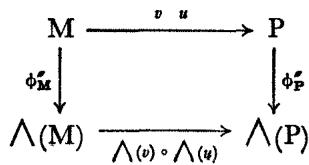
\includegraphics[keepaspectratio]{images/part003_3a522f8d.jpg}}

由于 \(\bigwedge (\mathbf{M})\) 包含 \(\mathbf{M} = \bigwedge^{1}(\mathbf{M}),\bigwedge (u)\) 有时称为 \(u\) 到 \(\bigwedge (\mathbf{M})\) 的典范扩张。限制 \(\bigwedge^n (u):\bigwedge^n (\mathbf{M})\to \bigwedge^n (\mathbf{N})\) 满足

\[
\bigwedge^ {n} (u) (x _ {1} \land x _ {2} \land \dots \land x _ {n}) = u (x _ {1}) \land u (x _ {2}) \land \dots \land u (x _ {n})\tag{4}
\]

（其中 \(x_{i}\in\mathbf{M}\) ），因为 \(\bigwedge(u)\) 是一个代数同态且 \(\bigwedge^{1}(u)=u\) ；限制 \(\bigwedge^{0}(u)\) 在 A 上是恒等映射。注意， \(\bigwedge^{n}(u)\) 是由 \(\mathsf{T}^{n}(u):\mathsf{T}^{n}(\mathbf{M})\to\mathsf{T}^{n}(\mathbf{N})\) 通过过渡到商而得到的。

命题 3. 若 \(u: \mathbf{M} \to \mathbf{N}\) 是满射 A-线性映射，则同态 \(\bigwedge(u): \bigwedge(\mathbf{M}) \to \bigwedge(\mathbf{N})\) 是满射的，且其核为 \(\bigwedge(\mathbf{M})\) 中由核 \(\mathbf{P} \subset \mathbf{M} \subset \bigwedge(\mathbf{M})\) （即 \(u\) 的核）生成的双边理想。

证明由 § 6，第 2 号，命题 4 的证明导出，只需将 S 换为 \(\bigwedge\) 并将 \(\mathfrak{J}'\) 换为 \(\mathfrak{J}''\) 。

若 \(u: \mathbf{M} \to \mathbf{N}\) 是单射线性映射， \(\bigwedge(\mathbf{u})\) 并不总是单射映射（§ 6，练习 3）（然而参见下文第 9 号，命题 12 的推论）。但当 \(u\) 是使得 \(u(\mathbf{M})\) 为 \(\mathbf{N}\) 的直因子的单射时，情况确实如此，且此时 \(\bigwedge(u)\) （同构于 \(\bigwedge(\mathbf{M})\) ）的像是 \(\bigwedge(\mathbf{N})\) 的直因子；其证明与关于 \(\mathbf{T}(u)\) 的类似断言的证明相同（§ 5，第 2 号），只需将 \(\mathbf{T}\) 换为 \(\bigwedge\) 。

命题 4. 设 N 和 P 是 A-模 M 的两个子模，使得它们的和 N + P 是 M 中的直和因子，且它们的交 N ∩ P 是 N 和 P 中的直和因子。则同态 \(\bigwedge(\mathrm{N}) \to \bigwedge(\mathrm{M})\) , \(\bigwedge(\mathrm{P}) \to \bigwedge(\mathrm{M})\) 和 \(\bigwedge(\mathrm{N} \cap \mathrm{P}) \to \bigwedge(\mathrm{M})\) ，即典范单射的典范扩张，是单射；若 \(\bigwedge(\mathrm{N})\) , \(\bigwedge(\mathrm{P})\) 和 \(\bigwedge(\mathrm{N} \cap \mathrm{P})\) 通过这些同态被等同于 \(\bigwedge(\mathrm{M})\) 的子代数，则

\[
\bigwedge (\mathbf {N} \cap \mathbf {P}) = \bigwedge (\mathbf {N}) \cap \bigwedge (\mathbf {P}).\tag{5}
\]

其证明由 § 5，第 2 号，命题 4 的证明导出，只需通篇将 T 换为 \(\bigwedge\) 。当 A 是域时，命题 4 的假设总是被 M 的任意子模 N, P 满足。

推论。设 K 是一个交换域，M 是 K 上的一个向量空间。对每个元素 \(z \in \bigwedge(\mathbf{M})\) ，存在 M 的一个最小向量子空间 N，使得 \(z \in \bigwedge(\mathbf{N})\) 且 N 是有限维的。

证明由 § 5，第 2 号，命题 4 的推论的证明导出，只需通篇将 T 换为 \(\bigwedge\) 。

N 称为 M 的与 \(\bigwedge(\mathbf{M})\) 的元素 z 相关联的向量子空间。
% semantic-fragments: legacy-input-seam
\relax{}
